%!TEX root = PhD_Thesis.tex
\chapter[Human-in-the-Loop Control]{Human-in-the-Loop Control of Ultrasound-Guided Needle Steering}

\section{Introduction}
The experimental results presented in Chapter 4 showed promising accuracy in autonomous targeting of the needle tip. While these tests were performed in biological tissues, they were completed in a bench-top setting, over a relatively small needle steering workspace. Early tests in a more realistic clinical environment---using a porcine cadaver in a simulated interventional radiology suite---revealed several problems preventing the direct application of our bench-top techniques. The mechanical 3D ultrasound transducer used in the previous section has limited field of view relative to the size of the liver, and any motion of the transducer invalidates all existing data. (In Section~\ref{sec:AutonomousControl} the transducer was clamped relative to the tissue sample.) External tracking systems can be used to increase the ultrasound's field of view by creating panoramic data, but this necessitates additional infrastructure. The appearance of the vibrating needle in Doppler ultrasound can be highly irregular in more realistic imaging arrangements. The Doppler approach still provides an indication of needle pose, but more sophisticated segmentation algorithms would be needed for autonomous control as in Section~\ref{sec:AutonomousControl}. Finally, visualization of 3D ultrasound data, needle pose, target location, etc. requires specialized software.

To allow closed-loop ultrasound-guided needle steering in a realistic clinical situation, we implemented our UKF estimation scheme using a different imaging approach. Specifically, we used freehand-3D ultrasound imaging, and manual localization of the steerable needle tip. 

This chapter is divided into three sections. Section~\ref{sec:HumanInTheLoopImplementation} describes the algorithmic, hardware, and software implementation of our human-in-the-loop approach. Section~\ref{sec:HumanInTheLoopValidation} describes experimental validation of our human-in-the-loop control approach, in bench-top and simulated clinical testing. Section~\ref{sec:HumanInTheLoopResults} presents the results.

\section{Implementation}
\label{sec:HumanInTheLoopImplementation}

\subsection{Robot and Steerable Needles}
\label{sec:NS2RobotAndNeedle}
Chapter 3 presented a new articulated-tip steerable needle that showed promising curvature results in biological tissue. Unfortunately, as discussed in that chapter, the plastic construction of the miniature hinges failed too frequently to be used in a simulated clinical setting. Chapter 6 discusses possible future improvements to the hinge design. In this chapter, we applied the exaggerated tip geometry suggested by the results of Chapter 3, but used a flexure tip, consisting of a rectangular Nitinol wire plastically deformed to the desired tip angle. This tip is able to pass through an introducer sheath, because of the large elastic range of Nitinol, and while returning to its bent shape inside tissue. This design does require duty cycle control to follow straight paths, and may increase tissue damage, unlike the articulated-tip needle. A similar flexure tip was previously proposed by Swaney et al.~\cite{Swaney2013}. Fig.~\ref{fig:NS2AndNeedle} shows the flexure tip steerable needle and the robot used to drive it in this chapter.

\begin{figure}[!ht]
\centering
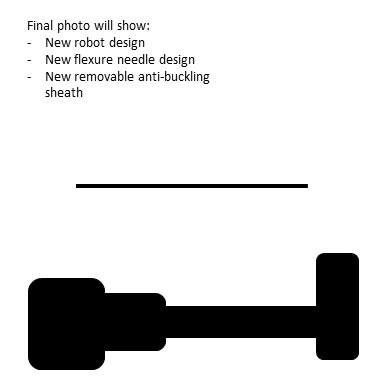
\includegraphics[width = 0.4\columnwidth]{./Images/Chapter5/NS2RobotAndNeedle/DRAFTNS2RobotAndNeedle.jpg}%
\caption[Robot and flexure-tip steerable needles]{Portable needle steering robot with positioning arm and handle, flexure-tip steerable with integrated anti-buckling sheath and connector fitting for introducer sheath.}
\label{fig:NS2AndNeedle}
\end{figure}  

\subsection{Control Modes}
Our implementation of human-in-the-loop control allows the user to select between joint-space control of the needle steering robot and task-space control of the needle tip position. In joint-space control, the user uses a 3D mouse (SpaceNavigator; 3Dconnexion, Boston, MA) to directly control the insertion and rotation of the needle steering robot's two DOF. Using a rate-control scheme, uniaxial displacement of the 3D mouse is mapped to insertion velocity, while uniaxial rotation of the 3D mouse is mapped to rotation speed. The remaining inputs of the 3D mouse are not used.

In task-space control, the user selects target positions directly in the live 2D ultrasound image using a tablet interface (Cintiq 13; Wacom Co., Vancouver, WA. The robot then steers the needle towards the target semi-autonomously, with feedback based on the output from the UKF estimation scheme described in Chapter 4. The estimator is updated without measurement feedback (i.e., based on the process model) at the ultrasound machine's native framerate. After every 10~mm of insertion, the system requires a tip position measurement, which the user provides by scanning over the needle tip and localizing it using the tablet interface. The estimation scheme is implemented exactly as described in Chapter 4 with two exceptions. First, the process and measurement noise levels were again experimentally characterized for the flexure needle and manual measurements, and the filter gains were adjusted accordingly. Second, the manual measurements only provided feedback on tip position, so tip orientation feedback was taken directly from the output of the estimator, with extremely low gain (high variance). This approach avoided practical computational issues related to matrix inversion and manipulation.

\begin{figure}[!t]
\centering
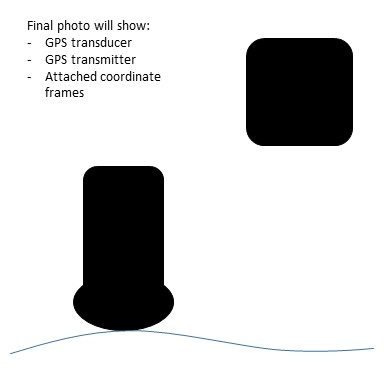
\includegraphics[width = 0.4\columnwidth]{./Images/Chapter5/Freehand3DUS/DRAFTFreehand3DUS.jpg}%
\caption[Freehand 3D ultrasound imaging arrangement]{Freehand 3D ultrasound imaging arrangement. The ultrasound transducer with integrated tracking element and electromagnetic tracking base station are depicted, along with the corresponding coordinate frames used to reconstruct the 3D pose of the 2D ultrasound image data.}
\label{fig:freehand3DUS}
\end{figure}  

\subsection{Freehand 3D Doppler Ultrasound Imaging}
As in the previous chapters, a SonixMDP ultrasound console (Ultrasonix Medical Corp., Richmond, Canada) was used for imaging. Unlike in the previous chapters, a 2D curvilinear transducer (C5-2/60) with an integrated electromagnetic tracking element was used. Fig.~\ref{fig:freehand3DUS} depicts this arrangement. The calibrated electromagnetic tracking system, branded as SonixGPS by Ultrasonix, allows the 3D context of the 2D ultrasound image data to be resolved in real time. 

As in Chapter 2, external vibrations were applied to the proximal end of the steerable needle shaft. However, in this chapter, a spring-loaded clip was used to attach a vibration motor (a miniature DC motor spinning a small eccentric mass) to the steerable needle shaft. Fig.~\ref{fig:Buzzer} shows the new vibration device. Compared to the integrated piezoelectric buzzer described in Chapter 2, this system has the advantages that is completely disposable if contaminated with bodily fluids, and it can be visually monitored during insertion and retraction to ensure good coupling. These characteristics were identified as necessary after early cadaver testing.

\begin{figure}[!t]
\centering
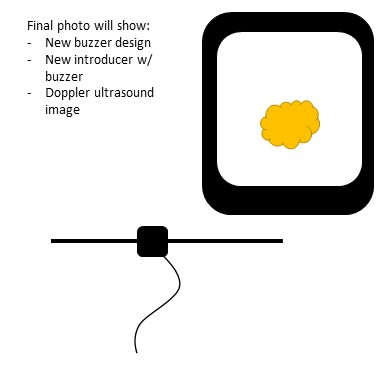
\includegraphics[width = 0.4\columnwidth]{./Images/Chapter5/Buzzer/DRAFTBuzzer.jpg}%
\caption[Disposable buzzer]{Disposable buzzer for ultrasound Doppler imaging. A 3D-printed spring-loaded clip attaches a vibration motor to the steerable needle shaft. The unit is battery powered and entirely disposable.}
\label{fig:Buzzer}
\end{figure}  

\subsection{Visualization and Control Software}
A custom graphical user interface (GUI) was developed using Qt for human-in-the-loop control. The GUI is shown in Fig.~\ref{fig:GUI}. The clinician user views both a live 2D ultrasound image streamed from the SonixMDP console, as well as a live 3D visualization of the robot pose, transducer pose, estimate, and target, as defined using the SonixGPS tracker. The GUI is optimized for a tablet interface. Controls allow the user to select between the two control modes (joint-space control and task-space control). The user can also use the tablet interface to set a the target point by clicking in the live 2D ultrasound image. Measurements of the steerable needle tip's position are similarly performed by clicking in the live 2D ultrasound image. 

\begin{figure}[!t]
\centering
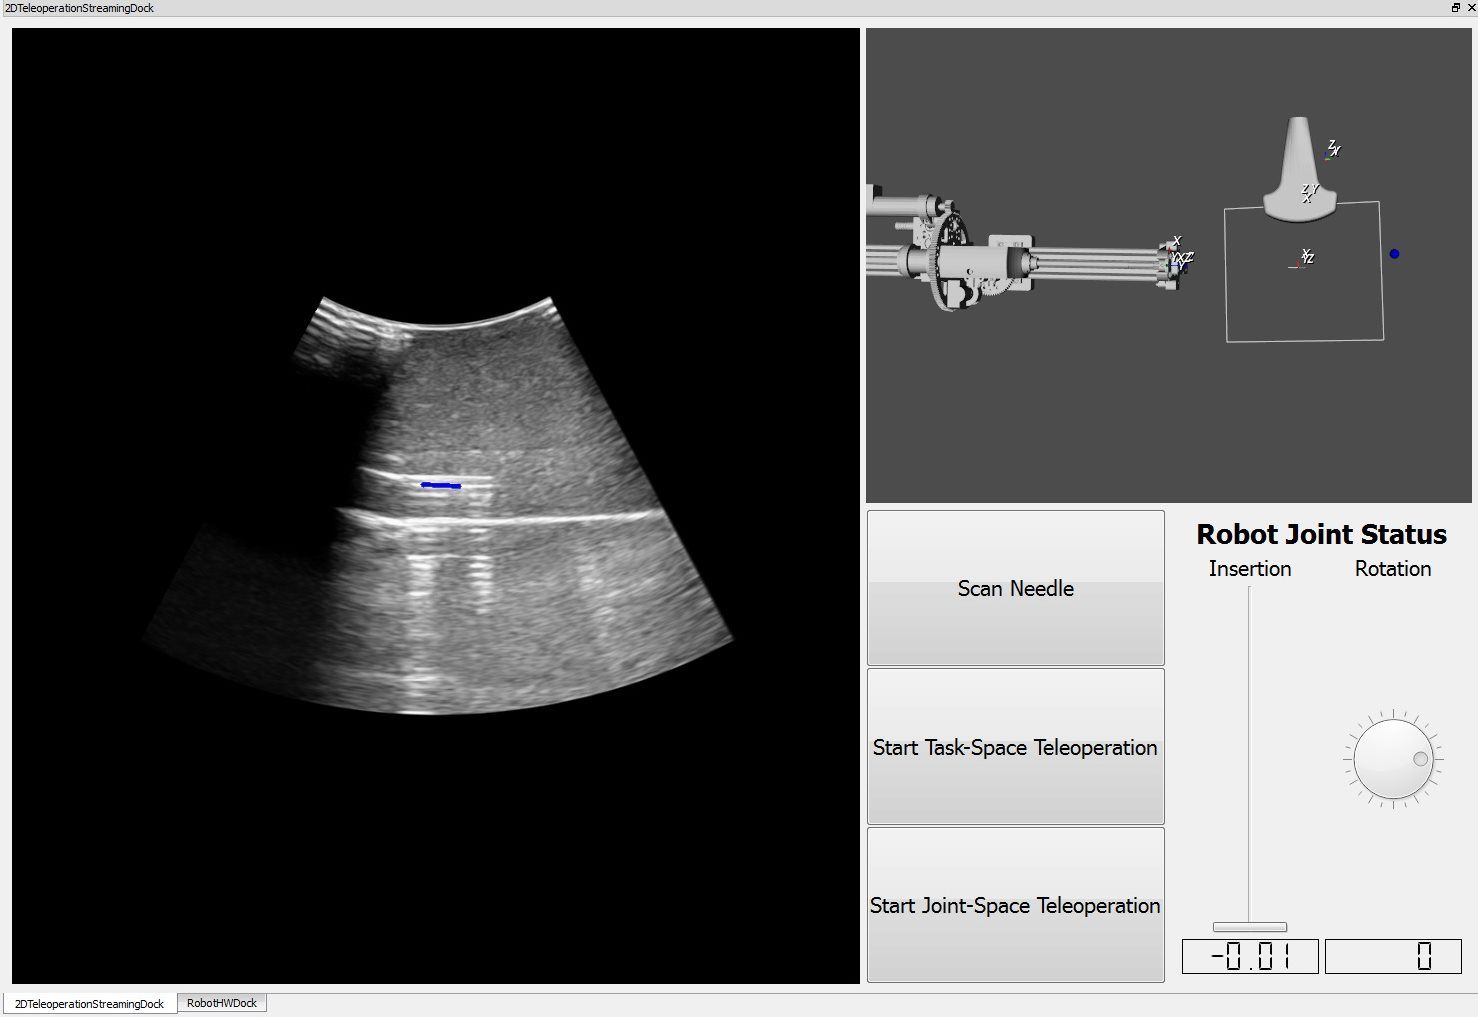
\includegraphics[width = 0.9\columnwidth]{./Images/Chapter5/GUI/GUI.jpg}%
\caption[Software interface]{Software interface for human-in-the-loop control. A screenshot shows the software during initial insertion of the robot, while the steerable needle tip is still within the introducer needle. Three panels are shown: (left) the live 2D ultrasound image with the current tip frame estimate over the hyperechoic needle shaft, (top right) the 3D visualization showing the ultrasound transducer pose, robot pose, tip frame estimate, and target (blue sphere), (bottom right) software control buttons and robot status readout.}
\label{fig:GUI}
\end{figure}  






\section{Validation Methods}
\label{sec:HumanInTheLoopValidation}

\subsection{Quantification of Process and Measurement Noise}
As in Chapter 4, we first quantified process noise and measurement noise using our new robot and imaging arrangement. Process noise was again quantified by using a magnetic tracking system to precisely measure the motion of a steerable needle tip during incremental insertion along constant curvature paths. In this testing, a flexure-tip steerable needle with $l = 10$~mm and $\alpha = 45$~degrees was used. The needle was inserted along a minimum-radius-of-curvature path at a constant insertion velocity of XX mm/s, and no rotation. The pose of the needle tip after each incremental step was compared with what was expected based on the previous pose and the process model. Although the insertion increment varied slightly due to software timing, it was generally about 0.2~mm. The needle was inserted along six paths, with 617 total measurements captured. The initial tip frame orientation was defined in the robot frame based on fixture geometry and the initial joint values $\theta$ and $\l$. Radius of curvature $\rho$ for the needle was also measured using the magnetic tracking data and the least-squares fitting approach described in Chapter~3. Data analysis was performed offline using Matlab. 

Measurement noise was quantified by comparing manual tip localization results from repeated freehand-3D ultrasound scans of steerable needles in porcine liver tissue. Five repeated measurements were performed at each tip position, with 200 total measurements over five needle insertions. For each measurement, the user scanned over the needle with the ultrasound transducer, and manually selected the location of the steerable needle tip using the tablet and stylus. Data analysis was again performed offline in Matlab.

\subsection{Accuracy of Estimation Scheme}

\subsection{Bench-Top Steering Experiments}

\subsection{Simulated Clinical Steering Experiments}


\section{Validation Results}
\label{sec:HumanInTheLoopResults}

\subsection{Quantification of Process and Measurement Noise}
Across 517 samples of process noise, the mean position error (in millimeters) and mean orientation error (in degrees) were \[{\overline{p}_{w}} = \begin{bmatrix} 0.03 &-1.68 &0.01 \end{bmatrix}^{\text{T}}, {\overline{r}_{w}} = \begin{bmatrix} 0.18 &-0.03 &0.08 \end{bmatrix}^{\text{T}}.\] To find the best-fit zero-mean Gaussian distribution to the process noise, we again reflected the measured noise vectors, resulting in a sample covariance of
\begin{align*}
{\hat{Q}} = \begin{bmatrix} 
\phantom{-}0.16 & \phantom{-}0.02 	&-0.04 & -0.13 & \phantom{-}1.47 & \phantom{-}3.41\\
\phantom{-}0.02 & \phantom{-}0.19 & -0.02 & -4.42 & \phantom{-}1.72 & -0.39 \\ 
-0.04 & -0.02 & \phantom{-}0.46 & -5.63 & \phantom{-}0.74 & -1.60 \\
-0.13 & -4.42 & -5.63 & \phantom{-}894.5 & \phantom{-}13.84 & \phantom{-}119.9 \\
\phantom{-}1.47 & \phantom{-}1.72 & \phantom{-}0.74 & \phantom{-}13.84 & \phantom{-}181.9 & \phantom{-}84.88 \\
\phantom{-}3.41 & -0.39 & -1.60 & \phantom{-}119.9 & \phantom{-}84.88 & \phantom{-}791.4\\ 
\end{bmatrix}.
\end{align*}

In the measurement noise experiment, we again assumed the mean of repeated localization at each tip pose was the true needle pose. NOT CORRECT YET
\begin{align*}
{\hat{R}} = \begin{bmatrix} 
\phantom{-}2.29 & \phantom{-}1.58 & \phantom{-}2.51 \\ 
\phantom{-}1.58 & \phantom{-}6.97 & \phantom{-}2.19 \\ 
\phantom{-}2.51 & \phantom{-}2.19 & \phantom{-}11.4 \\ 
\end{bmatrix}.
\end{align*}
